\documentclass[11pt,a4paper]{article}
\usepackage[utf8]{inputenc}
\usepackage[T1]{fontenc}
\usepackage{tgpagella}
\usepackage[spanish]{babel}
\usepackage{geometry}
\usepackage{booktabs}
\usepackage{xcolor}
\usepackage{titlesec}
\usepackage{fancyhdr}
\usepackage[parfill]{parskip}
\usepackage[expansion=false]{microtype}
\usepackage{hyperref}
\usepackage{setspace}
\usepackage{graphicx}
\usepackage{needspace}
\widowpenalty=10000
\clubpenalty=10000
\displaywidowpenalty=10000

\geometry{top=3.0cm,bottom=3.0cm,left=3.5cm,right=3.5cm}
\setlength{\parskip}{0.65em}
\setlength{\parindent}{0em}

\definecolor{azulai}{RGB}{30,80,140}
\definecolor{doradoai}{RGB}{140,90,0}
\definecolor{grisai}{RGB}{70,70,70}

\titleformat{\section}{\Large\bfseries\color{azulai}}{}{0em}{}[{\color{azulai}\titlerule[0.5pt]}]
\titlespacing*{\section}{0pt}{1.4em}{0.5em}

\titleformat{\subsection}{\large\bfseries\color{doradoai}}{}{0em}{}
\titlespacing*{\subsection}{0pt}{1.0em}{0.35em}

\titleformat{\subsubsection}{\normalsize\bfseries\color{grisai}}{}{0em}{}
\titlespacing*{\subsubsection}{0pt}{0.7em}{0.25em}

\pagestyle{fancy}\fancyhf{}
\rhead{\textcolor{grisai}{\small Virginia Riezu — Arquitectura Interna}}
\lhead{\textcolor{grisai}{\small Urano · Neptuno · Plutón}}
\cfoot{\textcolor{grisai}{\small\thepage}}
\renewcommand{\headrulewidth}{0.3pt}

\hypersetup{colorlinks=true,linkcolor=azulai,urlcolor=azulai}
\setstretch{1.25}
\tolerance=1500
\emergencystretch=4em

\begin{document}

% ── Portada ──────────────────────────────────────────────────────────────────
\begin{titlepage}
  \centering
  \vspace*{1.5cm}
  {\Huge\bfseries\color{azulai} Urano · Neptuno · Plutón}\\[0.5cm]
  {\large\color{grisai} Arquitectura Interna}\\[0.3cm]
  {\small\itshape\color{grisai} Procesos profundos de cambio, sensibilidad y transformación}\\[2cm]
  {\huge\color{doradoai} Virginia Riezu}\\[1.5cm]
  {\Large 06/09/1975 \quad 01:30}\\[0.3cm]
  {\Large Pamplona, España}\\[0.3cm]
  {\normalsize Lat: 42.8157° \quad Lon: -1.6522° \quad UTC+02:00}\\[0.3cm]
  {\normalsize Ascendente: Géminis 29°04' \quad
    MC: Piscis 3°22'}\\[2cm]
  \begin{tabular}{ll}
    \textbf{Urano:}   & Libra — Casa 5 29°54'  \\
    \textbf{Neptuno:} & Sagitario — Casa 6 9°05' \\
    \textbf{Plutón:}  & Libra — Casa 5 8°07' \\
  \end{tabular}\\[2cm]
  \vfill
  {\small Generado el 20/05/2026}
\end{titlepage}

\tableofcontents
\newpage

% ── Datos de referencia ───────────────────────────────────────────────────────
\section{Datos de referencia}

\begin{center}
\begin{tabular}{llll}
  \toprule
  \textbf{Planeta} & \textbf{Signo} & \textbf{Casa} & \textbf{Posición} \\
  \midrule
  Urano    & Libra   & 5   & 29°54'  \\
  Neptuno & Sagitario  & 6  & 9°05' \\
  Plutón  & Libra  & 5  & 8°07' \\
  Sol              & Virgo  & 4  & 12°46' \\
  Luna             & Virgo & 4 & 15°17' \\
  Ascendente       & Géminis          & ---                   & 29°04' \\
  Medio Cielo      & Piscis           & ---                   & 3°22' \\
  \bottomrule
\end{tabular}
\end{center}

\vspace{0.5cm}
\textbf{Aspectos relevantes:}

\begin{center}
\begin{tabular}{lllll}
  \toprule
  \textbf{Planeta 1} & \textbf{Asp.} & \textbf{Planeta 2} & \textbf{Tipo} & \textbf{Orbe} \\
  \midrule
  Plutón & conj & Mercurio & Conjunción & 0.2° \\
  Neptuno & sex & Mercurio & Sextil & 0.8° \\
  Neptuno & sex & Plutón & Sextil & 1.0° \\
  Urano & cua & Saturno & Cuadratura & 1.0° \\
  Urano & sex & Venus & Sextil & 1.6° \\
  Neptuno & cua & Sol & Cuadratura & 3.7° \\
  Neptuno & opo & Marte & Oposición & 3.8° \\
  Quirón & opo & Urano & Oposición & 4.4° \\
  Plutón & tri & Marte & Trígono & 4.7° \\
  Urano & opo & Júpiter & Oposición & 6.0° \\
  Neptuno & cua & Luna & Cuadratura & 6.2° \\
  \bottomrule
\end{tabular}
\end{center}

\begin{center}
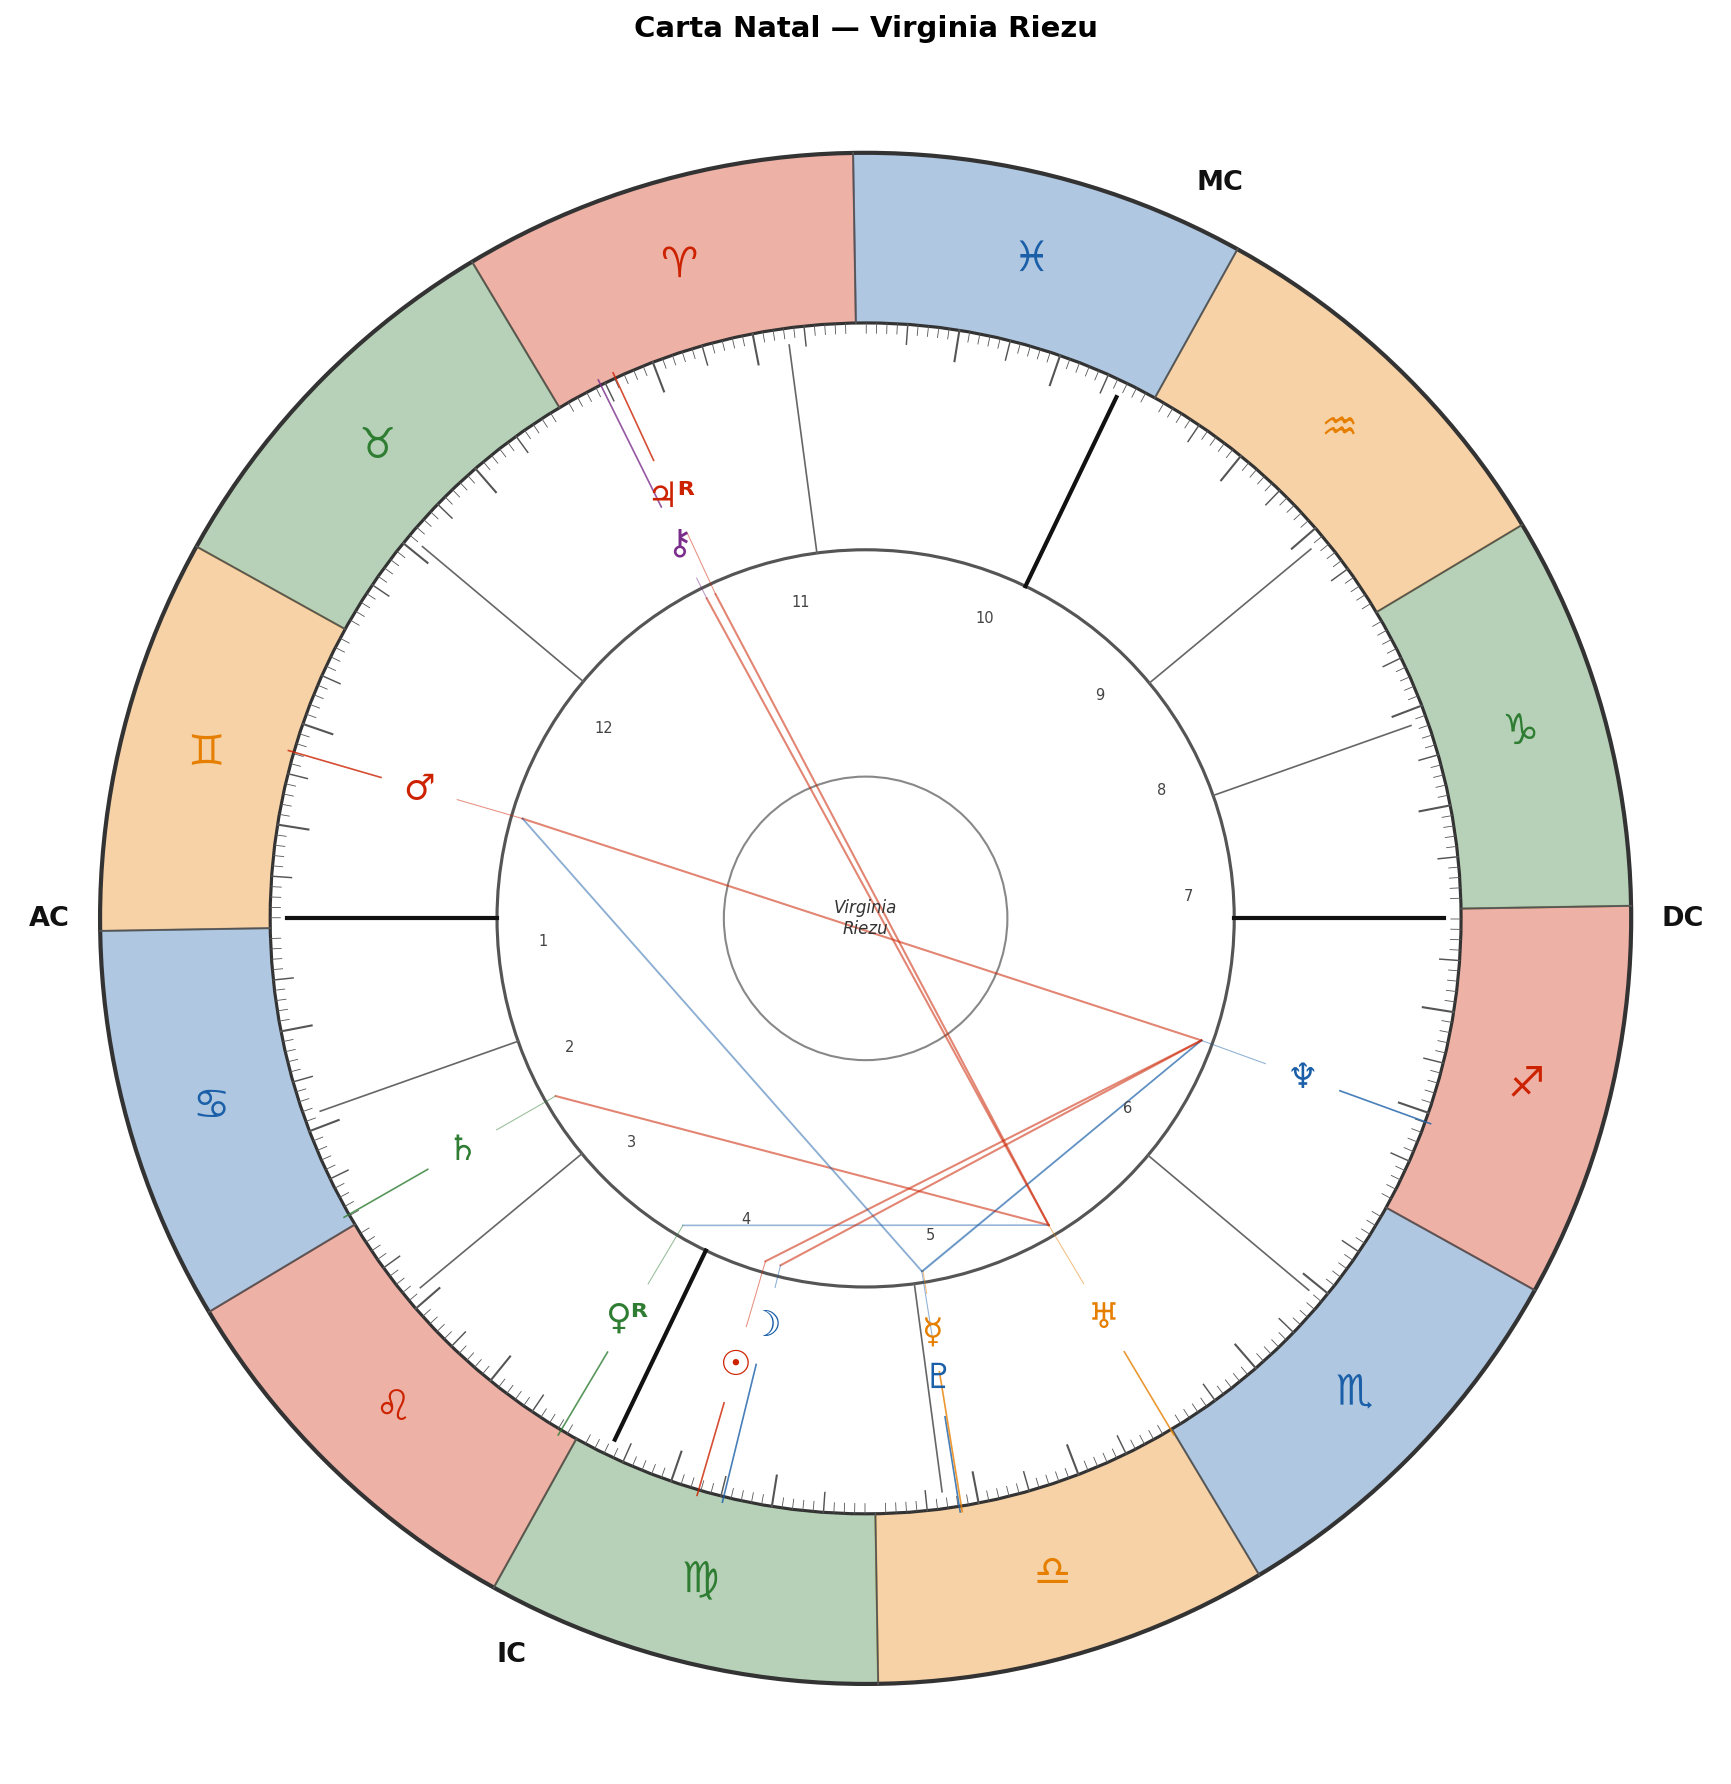
\includegraphics[width=0.72\textwidth]{Virginia_Riezu_rueda.png}
\end{center}

\Needspace{3\baselineskip}


% ── Interpretación ────────────────────────────────────────────────────────────
\section{Interpretación — Arquitectura Interna}

\begin{center}
{\small\itshape
No se trata de describir la personalidad. Se trata de mostrar qué procesos\\
de cambio, sensibilidad y transformación pueden activarse en tu vida.
}
\end{center}

\vspace{0.8cm}
\Needspace{5\baselineskip}

% ── 1. Marco general ──────────────────────────────────────────────────────────
\subsection{1. Marco general}

Urano, Neptuno y Plutón no describen lo más cotidiano o visible de tu carta. Muestran procesos más profundos, menos controlables, que pueden modificar tu forma de vivir, sostenerte y atravesar determinadas etapas.

Urano en Libra, Casa 5: muestra dónde aparecen cambios, interrupciones o necesidad de libertad. Cuando se activa, algo que antes funcionaba puede dejar de hacerlo igual.
Neptuno en Sagitario, Casa 6: muestra dónde los límites se vuelven más sensibles, difusos o permeables. Cuando se activa, algo que parecía claro puede perder forma.
Plutón en Libra, Casa 5: muestra dónde aparecen procesos intensos de transformación. Cuando se activa, algo que se sostenía de una manera ya no puede seguir igual.

Aspectos activos con planetas personales: Urano–Venus en sextil (orbe 1.59°), Neptuno–Sol en cuadratura (orbe 3.69°), Neptuno–Luna en cuadratura (orbe 6.19°), Neptuno–Mercurio en sextil (orbe 0.78°), Neptuno–Marte en oposición (orbe 3.76°), Plutón–Mercurio en conjunción (orbe 0.2°), Plutón–Marte en trígono (orbe 4.74°).

\vspace{0.8cm}
\Needspace{5\baselineskip}


% ── 2. Urano ──────────────────────────────────────────────────────────────────
\subsection{2. Urano — Ruptura y cambio de patrón}

\subsubsection*{Urano en Libra — Casa 5}

Urano en Libra muestra necesidad de libertad dentro de los vínculos y dificultad para sostener relaciones demasiado rígidas o previsibles. Los cambios suelen aparecer cuando la forma de relacionarte deja de sentirse viva o auténtica.

Puede haber giros importantes en relaciones, acuerdos o maneras de vincularte. A veces necesitas tomar distancia para poder recuperar claridad sobre lo que realmente quieres compartir.

El aprendizaje pasa por construir relaciones donde exista espacio para el cambio sin que cada transformación implique una ruptura.

Urano en Casa 5 muestra necesidad de expresarte de forma libre, auténtica y poco convencional. Puede costarte sostener formas creativas demasiado previsibles o repetitivas.

A veces aparecen etapas de mucha inspiración seguidas de cortes bruscos o cambios de dirección. También puede haber giros importantes en la forma de vivir el deseo, la creatividad o la necesidad de reconocimiento.

El aprendizaje está en sostener la creatividad sin necesitar romper constantemente con lo que estabas construyendo.

Urano en sextil a Venus facilita introducir renovación y movimiento en las relaciones de manera bastante consciente. Existe capacidad para transformar vínculos sin necesidad de ruptura permanente.

Las nuevas experiencias afectivas suelen ayudarte a comprender mejor qué necesitas realmente.

El aprendizaje está en permitir cambios graduales antes de llegar al corte brusco.

\vspace{0.8cm}
\Needspace{5\baselineskip}

% ── 3. Neptuno ────────────────────────────────────────────────────────────────
\subsection{3. Neptuno — Disolución y pérdida de forma}

\subsubsection*{Neptuno en Sagitario — Casa 6}

Neptuno en Sagitario puede hacer que busques sentido, dirección o verdad en lugares que después resultan menos sólidos de lo que parecían. A veces necesitas creer en algo para sentir orientación, incluso cuando todavía no está claro.

Puede haber idealización de caminos, proyectos, filosofías o personas que parecen ofrecer amplitud o propósito. También puedes cambiar varias veces de dirección buscando una referencia más auténtica.

El aprendizaje está en desarrollar una visión más consciente sin perder apertura ni capacidad de inspiración.

Neptuno en Casa 6 vuelve más difusos los límites relacionados con trabajo, hábitos y funcionamiento cotidiano. Puede costarte mantener rutinas claras o reconocer a tiempo cuándo algo te está agotando.

A veces hay confusión en horarios, organización o formas de cuidar el cuerpo y la energía. También puedes absorber demasiado del ambiente laboral o de las exigencias externas.

El aprendizaje está en desarrollar hábitos más conscientes y sostenibles sin rigidizarte.

Neptuno en cuadratura al Sol genera tensión entre necesidad de claridad y tendencia a la dispersión o la confusión. Una parte de ti busca dirección definida, mientras otra necesita abrirse a algo más amplio o difícil de concretar.

Puede haber sensación de desorientación, dificultad para sostener decisiones o etapas donde lo que parecía claro deja de tener forma.

El aprendizaje pasa por reconocer antes cuándo algo ya no tiene suficiente verdad para seguir sosteniéndolo.

Neptuno en cuadratura a la Luna genera tensión entre necesidad de estabilidad emocional y tendencia a la dispersión o la permeabilidad emocional. Una parte de ti busca seguridad y otra absorbe constantemente lo que ocurre alrededor.

Puede haber dificultad para entender lo que sientes realmente, idealización emocional o sensación de agotamiento cuando no existen suficientes límites.

El aprendizaje pasa por cuidar mejor tu energía emocional sin endurecerte internamente.

Neptuno en sextil a Mercurio facilita conectar intuición y pensamiento de forma bastante natural. Existe capacidad para abrir nuevas perspectivas sin perder completamente claridad.

La imaginación y la sensibilidad suelen enriquecer mucho la manera de pensar y comunicar.

El aprendizaje está en sostener más foco y continuidad en las ideas.

Neptuno en oposición a Marte intensifica la tensión entre impulso de acción y tendencia a perder dirección o límites claros. A veces quieres avanzar con fuerza pero algo interno disuelve rápidamente la motivación o el objetivo.

Puede haber dificultad para sostener continuidad en la acción o sensación de moverte desde impulsos difíciles de concretar.

El aprendizaje está en encontrar una forma de actuar más consciente y conectada con lo que realmente tiene sentido para ti.

\vspace{0.8cm}
\Needspace{5\baselineskip}

% ── 4. Plutón ─────────────────────────────────────────────────────────────────
\subsection{4. Plutón — Intensidad y transformación profunda}

\subsubsection*{Plutón en Libra — Casa 5}

Plutón en Libra intensifica profundamente los vínculos y la necesidad de equilibrio real en las relaciones. Las transformaciones suelen aparecer a través de acuerdos, rupturas o dinámicas relacionales difíciles de sostener superficialmente.

Puede haber miedo a perder vínculos importantes, relaciones muy intensas o dificultad para mantener relaciones donde no existe reciprocidad verdadera.

El aprendizaje pasa por construir vínculos más honestos y profundos sin quedar atrapade en dinámicas de dependencia o control.

Plutón en Casa 5 intensifica la creatividad, el deseo y la necesidad de expresarte de forma auténtica. Las experiencias relacionadas con amor, creación o reconocimiento suelen vivirse con mucha profundidad.

Puede haber intensidad emocional en vínculos afectivos, necesidad fuerte de expresión o dificultad para crear desde un lugar ligero o superficial.

El aprendizaje está en expresar lo que eres sin convertir cada experiencia emocional en una lucha de intensidad.

Plutón en conjunción con Mercurio intensifica muchísimo la mente y la necesidad de comprender lo que hay debajo de las apariencias. Te cuesta quedarte en explicaciones superficiales.

Puede haber pensamientos obsesivos, gran capacidad de análisis o necesidad de investigar profundamente determinados temas.

El aprendizaje está en permitir profundidad mental sin quedar atrapade en análisis constantes.

Plutón en trígono a Marte facilita integrar intensidad, voluntad y capacidad de transformación. La energía suele sentirse fuerte, enfocada y resistente.

Existe capacidad para atravesar situaciones difíciles sin perder completamente dirección ni fuerza interna.

El aprendizaje pasa por usar esa potencia de manera constructiva y no únicamente desde exigencia o control.

\vspace{0.8cm}
\Needspace{5\baselineskip}

% ── 5. Integración ────────────────────────────────────────────────────────────
\subsection{5. Integración — Las tres fuerzas en tu carta}

Urano, Neptuno y Plutón actúan de formas distintas y no siempre coordinadas. Urano en Libra, Casa 5, muestra dónde aparecen cambios, interrupciones o necesidad de libertad. Cuando se activa, algo que antes funcionaba puede dejar de hacerlo igual. Neptuno en Sagitario, Casa 6, muestra dónde los límites se vuelven más sensibles, difusos o difíciles de sostener. Cuando se activa, algo que parecía claro puede perder forma. Plutón en Libra, Casa 5, muestra dónde aparecen procesos intensos de transformación. Cuando se activa, algo que sostenías de una manera ya no puede seguir igual.

Neptuno en Sagitario muestra una sensibilidad especial en ciertas áreas de tu vida: tiendes a desbordarte por exceso de impulso o dificultad para frenar a tiempo. Urano en Libra muestra cómo suelen producirse los cambios importantes: los cambios aparecen cuando cambia tu manera de pensar o comprender las cosas. Plutón en Libra concentra la intensidad en procesos que no pueden quedarse igual indefinidamente: determinadas experiencias terminan empujándote a transformar algo en profundidad.

En determinados momentos, estas tres fuerzas pueden activarse de forma encadenada. Urano en Libra suele aparecer primero: tu manera de pensar o entender una situación cambia bruscamente. Después, Neptuno en Sagitario puede hacer que aparezca sensación de confusión, pérdida de claridad o dificultad para entender bien qué está pasando: la energía pierde dirección y cuesta saber hacia dónde moverte. Finalmente, Plutón en Libra concentra la intensidad en aquello que ya no puede seguir igual: la intensidad se concentra en pensamientos, conversaciones o formas de comprender la vida. Por eso, determinadas etapas pueden sentirse especialmente intensas: no estás viviendo una sola cosa, sino varios procesos moviéndose al mismo tiempo.

\vspace{0.8cm}
\Needspace{5\baselineskip}

% ── 6. Orientación ────────────────────────────────────────────────────────────
\subsection{6. Orientación}

\subsubsection*{Cuando Urano está activo}
Urano suele activarse cuando: cambia bruscamente tu manera de pensar, comprender o comunicar algo. Esto suele sentirse especialmente en temas relacionados con la Casa 5.

\subsubsection*{Cuando Neptuno está activo}
Neptuno suele activarse cuando: pierdes claridad sobre hacia dónde quieres dirigirte. Esto suele sentirse especialmente en temas relacionados con la Casa 6.

\subsubsection*{Cuando Plutón está activo}
Plutón suele activarse cuando: determinados pensamientos o conversaciones adquieren mucha intensidad y profundidad. Esto suele sentirse especialmente en temas relacionados con la Casa 5.

\subsubsection*{Cuando no se reconocen}
Cuando estos procesos no se reconocen, es fácil vivirlos únicamente como problemas externos o mala suerte. Sin embargo, muchas veces están mostrando que algo necesita cambiar, redefinirse o transformarse más profundamente.

Intentar sostener exactamente igual algo que internamente ya está cambiando suele generar más desgaste, más confusión o más sensación de bloqueo.

\vspace{0.6cm}
Si estos procesos se ignoran durante mucho tiempo, suelen intensificarse. Urano puede traer cambios cada vez más bruscos. Neptuno puede aumentar la sensación de confusión, desgaste o pérdida de claridad. Plutón puede concentrar tanta intensidad que determinadas situaciones ya no puedan seguir sosteniéndose igual.

Por eso, reconocer antes lo que está cambiando suele ayudar a atravesar estas etapas con más consciencia y menos ruptura.

\vspace{1cm}
\begin{center}
{\small\itshape\color{grisai}
La astrología se usa aquí como lenguaje simbólico de observación, no como definición de la persona.\
Este documento es una aproximación funcional, no un diagnóstico.
}
\end{center}

\end{document}
